\section{Signal Regions}
\label{sec:Optimization}

%The type-III seesaw signal comes both with 3 and 4 (or more) leptons as well as with and without OSSF pairs, which in turn may have an invariant mass that is compatible with \Z production. This lays the foundation for our binning scheme.

Backgrounds can be tamed by binning in appropriate quantities. Given the relatively high signal lepton momenta due to the large masses of the parent particles, cutting on $L_\textrm{T}$, the scalar lepton \pt sum, may be a good idea. This is especially true for decay modes like $\Sigma^\pm \to \ell^\pm \Z \to \ell^\pm ~ \ell^{\prime \pm} \ell^{\prime \mp}$ where the heavy fermion mass is transformed into the lepton momenta. However, such an $L_\textrm{T}$ cut acts at the expense of the signal efficiency in other modes like $\Sigma^0 \to \PH \nu \to \PW\PW\nu$, where lepton \pt's are somewhat lower because the intermediate bosons may be off-shell, and the neutrinos carry away some of the momentum that appears as missing transverse energy (\MET). However, we can still achieve high efficiency by using $L_\textrm{T} + \MET$ instead, which we found suitable for signal selection and background rejection for both of the described channel types. The effectiveness of this variable is shown in Fig.~\ref{fig:Optimization}. We find that lepton \pt binning alone gives about 20\,\% worse signal-to-background ratios in the most sensitive signal regions.

\begin{figure}
\begin{center}
	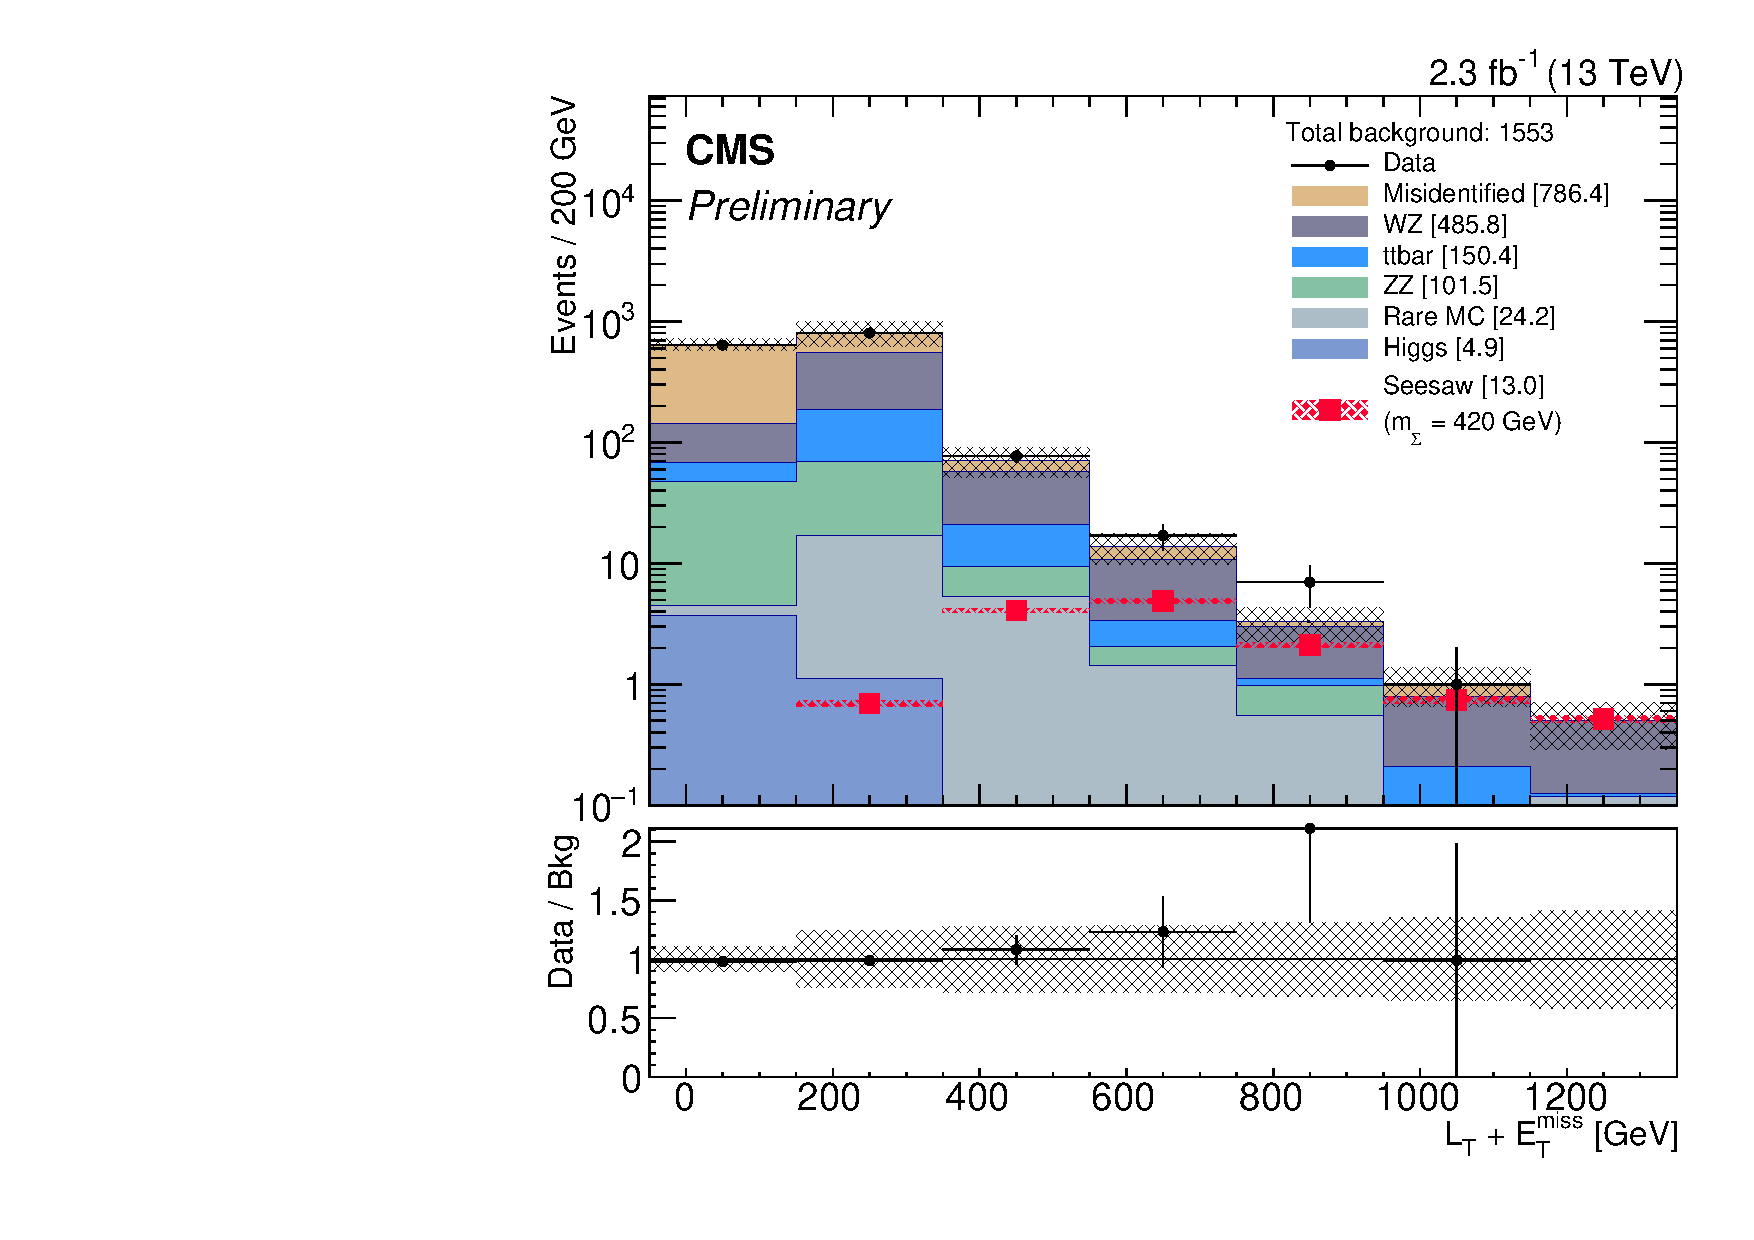
\includegraphics[width=.7\textwidth]{Optimization/LT+MET}
	\caption{$L_\textrm{T} + \MET$ distribution after event selection cuts from Sec.~\ref{sec:Selection}, to illustrate the signal separation power of this variable (last bin includes overflow). Backgrounds are described in Sec.~{\ref{sec:backgrounds}}. The signal ($m_\Sigma = 420\,\GeV$, sum of all production and decay modes) is shown as white square dots with a pink hashed uncertainty band. The background uncertainty is specified by the gray band. Uncertainty bands include both statistical and systematic uncertainties. Numbers in square brackets denote the number of events contributed by each process.
	\label{fig:Optimization}}
\end{center}
\end{figure}

The optimum requirement on $L_\textrm{T} + \MET$ depends on the mass of the heavy fermions. In order to separate the signal as best as possible from the background, we categorize the data in bins of $L_\textrm{T} + \MET$, regardless of the particle mass. We use 4 bins of width 200\,\GeV starting at 350\,\GeV, plus an overflow bin. Below 350\,\GeV, the amount of signal is insignificant in comparison to the background.

We remove any overlap with background control regions by explicitly vetoing the control region selections. Furthermore, we discard the below-\Z trilepton region and the four-lepton region without an OSSF pair because, with the given amount of luminosity, they contain a neglibile amount of signal and thus do not contribute to the sensitivity.

As a result, we have four $L_\textrm{T} + \MET$ distributions, depending on the lepton properties: 3 leptons without OSSF pair, 3 leptons with OSSF pair on-\Z, 3 leptons with OSSF pair above-\Z, and 4 leptons with at least one OSSF pair. Each distributions begins at 350\,\GeV and reaches to 1150\,\GeV in steps of 200\,\GeV. We add an overflow bin for $L_\textrm{T} + \MET > 1150\,\GeV$ so that that there are five bins per distribution, giving a total of 20 signal regions.

%The resulting set of 20 signal regions is described in Table~\ref{tab:SR}.

%\begin{table}[h]
%\centering
%\caption{Signal Regions. Overlap with control regions removed everywhere.} \label{tab:SR}
%\begin{tabular}{c l c }
%\hline\hline
%$n_\textrm{leptons}$ & OSSF pair & $L_\textrm{T} + \MET$ [GeV]\\
%\hline
%3 & & \\
% & none & \multirow{3}{*}{\rotatebox{9}{350..1150 in steps of 200, plus overflow}} \\
% & on-\Z & \\
% & above-\Z & \\
%\hline
%$\geq 4$ & $\geq 1$ & 350..1150 in steps of 200, plus overflow \\
%\end{tabular}
%\end{table}
